\documentclass[conference,letterpaper]{IEEEtran}
\IEEEoverridecommandlockouts
\usepackage{cite}
\usepackage{amsmath,amssymb}
\usepackage{graphicx}
\usepackage{booktabs}
\usepackage{array}
\usepackage{xcolor}
\usepackage{url}
\usepackage[hidelinks]{hyperref}

% Every result below is a macro generated by make_numbers.py from the
% evaluation outputs; nothing is typed by hand.
% AUTO-GENERATED by make_numbers.py — do not edit by hand
% source: ../final2
\newcommand{\Pilot}{0}
\newcommand{\PilotNote}{}
\newcommand{\NSubj}{23}
\newcommand{\NRec}{160}
\newcommand{\NSz}{194}
\newcommand{\NHours}{220}
\newcommand{\NColdStart}{15}
\newcommand{\NRecAll}{165}
\newcommand{\NSzAll}{198}
\newcommand{\NHoursAll}{225}
\newcommand{\PyBSens}{5.7\%}
\newcommand{\PyBDet}{11}
\newcommand{\PyBCI}{2--12\%}
\newcommand{\PyBMacro}{10.0\%}
\newcommand{\PyBMacroCI}{3--18\%}
\newcommand{\PyBFAh}{0.32}
\newcommand{\PyBFAday}{8}
\newcommand{\PyBFACI}{0.20--0.48}
\newcommand{\PyBLat}{26.3}
\newcommand{\PyASens}{21.1\%}
\newcommand{\PyADet}{41}
\newcommand{\PyACI}{14--29\%}
\newcommand{\PyAMacro}{25.4\%}
\newcommand{\PyAMacroCI}{15--36\%}
\newcommand{\PyAFAh}{2.82}
\newcommand{\PyAFAday}{68}
\newcommand{\PyAFACI}{2.00--3.86}
\newcommand{\PyALat}{28.4}
\newcommand{\FwBSens}{75.3\%}
\newcommand{\FwBDet}{146}
\newcommand{\FwBCI}{60--94\%}
\newcommand{\FwBMacro}{87.6\%}
\newcommand{\FwBMacroCI}{79--95\%}
\newcommand{\FwBFAh}{18.29}
\newcommand{\FwBFAday}{439}
\newcommand{\FwBFACI}{15.19--21.21}
\newcommand{\FwBLat}{14.5}
\newcommand{\DevASens}{52.1\%}
\newcommand{\DevADet}{101}
\newcommand{\DevACI}{36--74\%}
\newcommand{\DevAMacro}{68.6\%}
\newcommand{\DevAMacroCI}{54--82\%}
\newcommand{\DevAFAh}{0.97}
\newcommand{\DevAFAday}{23}
\newcommand{\DevAFACI}{0.71--1.31}
\newcommand{\DevALat}{22.0}
\newcommand{\DevBSens}{41.8\%}
\newcommand{\DevBDet}{81}
\newcommand{\DevBCI}{26--65\%}
\newcommand{\DevBMacro}{59.5\%}
\newcommand{\DevBMacroCI}{44--74\%}
\newcommand{\DevBFAh}{0.46}
\newcommand{\DevBFAday}{11}
\newcommand{\DevBFACI}{0.25--0.77}
\newcommand{\DevBLat}{23.0}
\newcommand{\DevCSens}{28.4\%}
\newcommand{\DevCDet}{55}
\newcommand{\DevCCI}{15--49\%}
\newcommand{\DevCMacro}{46.1\%}
\newcommand{\DevCMacroCI}{30--62\%}
\newcommand{\DevCFAh}{0.16}
\newcommand{\DevCFAday}{4}
\newcommand{\DevCFACI}{0.05--0.32}
\newcommand{\DevCLat}{29.0}
\newcommand{\LlASens}{25.3\%}
\newcommand{\LlADet}{49}
\newcommand{\LlACI}{15--42\%}
\newcommand{\LlAMacro}{40.1\%}
\newcommand{\LlAMacroCI}{26--55\%}
\newcommand{\LlAFAh}{1.04}
\newcommand{\LlAFAday}{25}
\newcommand{\LlAFACI}{0.72--1.35}
\newcommand{\LlALat}{32.0}
\newcommand{\LlBSens}{21.6\%}
\newcommand{\LlBDet}{42}
\newcommand{\LlBCI}{11--38\%}
\newcommand{\LlBMacro}{35.8\%}
\newcommand{\LlBMacroCI}{21--50\%}
\newcommand{\LlBFAh}{0.35}
\newcommand{\LlBFAday}{8}
\newcommand{\LlBFACI}{0.23--0.51}
\newcommand{\LlBLat}{24.5}
\newcommand{\FuASens}{40.2\%}
\newcommand{\FuADet}{78}
\newcommand{\FuACI}{24--64\%}
\newcommand{\FuAMacro}{56.0\%}
\newcommand{\FuAMacroCI}{41--70\%}
\newcommand{\FuAFAh}{0.96}
\newcommand{\FuAFAday}{23}
\newcommand{\FuAFACI}{0.67--1.27}
\newcommand{\FuALat}{21.5}
\newcommand{\TwoDevASens}{52.1\%}
\newcommand{\TwoDevADet}{101}
\newcommand{\TwoDevACI}{36--74\%}
\newcommand{\TwoDevAMacro}{68.6\%}
\newcommand{\TwoDevAMacroCI}{54--82\%}
\newcommand{\TwoDevAFAh}{0.95}
\newcommand{\TwoDevAFAday}{23}
\newcommand{\TwoDevAFACI}{0.69--1.31}
\newcommand{\TwoDevALat}{23.0}
\newcommand{\TwoDevBSens}{38.1\%}
\newcommand{\TwoDevBDet}{74}
\newcommand{\TwoDevBCI}{24--61\%}
\newcommand{\TwoDevBMacro}{57.3\%}
\newcommand{\TwoDevBMacroCI}{41--73\%}
\newcommand{\TwoDevBFAh}{0.37}
\newcommand{\TwoDevBFAday}{9}
\newcommand{\TwoDevBFACI}{0.23--0.55}
\newcommand{\TwoDevBLat}{27.0}
\newcommand{\NeASens}{52.1\%}
\newcommand{\NeADet}{101}
\newcommand{\NeACI}{36--74\%}
\newcommand{\NeAMacro}{68.6\%}
\newcommand{\NeAMacroCI}{54--82\%}
\newcommand{\NeAFAh}{0.97}
\newcommand{\NeAFAday}{23}
\newcommand{\NeAFACI}{0.71--1.31}
\newcommand{\NeALat}{22.0}
\newcommand{\NeBSens}{41.8\%}
\newcommand{\NeBDet}{81}
\newcommand{\NeBCI}{26--65\%}
\newcommand{\NeBMacro}{59.5\%}
\newcommand{\NeBMacroCI}{44--74\%}
\newcommand{\NeBFAh}{0.46}
\newcommand{\NeBFAday}{11}
\newcommand{\NeBFACI}{0.25--0.77}
\newcommand{\NeBLat}{23.0}
\newcommand{\DevASensWarm}{54.2\%}
\newcommand{\DevASzWarm}{179}
\newcommand{\DevBSensWarm}{43.6\%}
\newcommand{\DevBSzWarm}{179}
\newcommand{\DevAR}{1.25}
\newcommand{\DevAD}{20}
\newcommand{\DevAModeCount}{22}
\newcommand{\DevAFolds}{23}
\newcommand{\DevBR}{1.5}
\newcommand{\DevBD}{20}
\newcommand{\DevBModeCount}{20}
\newcommand{\DevBFolds}{23}
\newcommand{\NestedDev}{69}
\newcommand{\NestedAll}{69}
\newcommand{\PyBNull}{1.6\%}
\newcommand{\PyBNullNF}{3.1\%}
\newcommand{\PyBNullP}{$p{=}1{\times}10^{-3}$}
\newcommand{\PyANull}{12.8\%}
\newcommand{\PyANullNF}{16.5\%}
\newcommand{\PyANullP}{$p{=}0.002$}
\newcommand{\FwBNull}{56.6\%}
\newcommand{\FwBNullNF}{61.3\%}
\newcommand{\FwBNullP}{$p{=}1{\times}10^{-3}$}
\newcommand{\DevANull}{6.5\%}
\newcommand{\DevANullNF}{9.3\%}
\newcommand{\DevANullP}{$p{=}1{\times}10^{-3}$}
\newcommand{\DevBNull}{3.9\%}
\newcommand{\DevBNullNF}{6.2\%}
\newcommand{\DevBNullP}{$p{=}1{\times}10^{-3}$}
\newcommand{\LlANull}{4.8\%}
\newcommand{\LlANullNF}{7.2\%}
\newcommand{\LlANullP}{$p{=}1{\times}10^{-3}$}
\newcommand{\NPerm}{1000}
\newcommand{\ShipNullMaxP}{0.002}
\newcommand{\TestDevPyP}{$p{=}6{\times}10^{-5}$}
\newcommand{\TestDevPyBetter}{21}
\newcommand{\TestDevPyWorse}{0}
\newcommand{\TestDevPyTies}{2}
\newcommand{\TestDevPyN}{23}
\newcommand{\TestDevPyAnyP}{$p{=}7{\times}10^{-5}$}
\newcommand{\TestDevPyAnyBetter}{20}
\newcommand{\TestDevPyAnyWorse}{1}
\newcommand{\TestDevPyAnyTies}{2}
\newcommand{\TestDevPyAnyN}{23}
\newcommand{\TestDevLlP}{$p{=}7{\times}10^{-4}$}
\newcommand{\TestDevLlBetter}{15}
\newcommand{\TestDevLlWorse}{0}
\newcommand{\TestDevLlTies}{8}
\newcommand{\TestDevLlN}{23}
\newcommand{\FoldDevPy}{7}
\newcommand{\AucLL}{0.70}
\newcommand{\AucLLCase}{0.79}
\newcommand{\AucDAR}{0.51}
\newcommand{\AucDARCase}{0.58}
\newcommand{\AucHFE}{0.40}
\newcommand{\AucHFECase}{0.41}
\newcommand{\AucFW}{0.70}
\newcommand{\AucFWCase}{0.83}
\newcommand{\ArtIctal}{0.01\%}
\newcommand{\ArtInter}{0.01\%}
\newcommand{\PyBSensLowGain}{0.0\%}
\newcommand{\PyBSensHighGain}{13.4\%}
\newcommand{\PyBFAhLowGain}{0.24}
\newcommand{\PyBFAhHighGain}{1.59}
\newcommand{\FwBFAhLowGain}{7.36}
\newcommand{\FwBFAhHighGain}{24.37}
\newcommand{\MainTableBody}{%
Analyzer, BLACKOUT (shipped) & 11/194 & 5.7\% [2--12] & 10.0\% & 0.32 & 26.3 & 1.6\% \\
Analyzer, any alarm (shipped) & 41/194 & 21.1\% [14--29] & 25.4\% & 2.82 & 28.4 & 12.8\% \\
Firmware, BLACKOUT (shipped) & 146/194 & 75.3\% [60--94] & 87.6\% & 18.29 & 14.5 & 56.6\% \\
\midrule
LL-BR, $\le$1 FA/h & 49/194 & 25.3\% [15--42] & 40.1\% & 1.04 & 32.0 & 4.8\% \\
FUSE-BR, $\le$1 FA/h & 78/194 & 40.2\% [24--64] & 56.0\% & 0.96 & 21.5 & -- \\
\textbf{DEV-BR, $\le$1 FA/h} & 101/194 & 52.1\% [36--74] & 68.6\% & 0.97 & 22.0 & 6.5\% \\
\textbf{DEV-BR, $\le$0.5 FA/h} & 81/194 & 41.8\% [26--65] & 59.5\% & 0.46 & 23.0 & 3.9\% \\
\textbf{DEV-BR, $\le$0.2 FA/h} & 55/194 & 28.4\% [15--49] & 46.1\% & 0.16 & 29.0 & -- \\
}
\newcommand{\AblationTableBody}{%
\textbf{reference} (300 s, lag 30 s, median) & 52.1\% / 0.97 & 41.8\% / 0.46 \\
no lag (0 s) & 50.5\% / 0.79 & 34.5\% / 0.42 \\
lag 10 s & 51.0\% / 0.87 & 40.7\% / 0.45 \\
lag 60 s & 47.9\% / 0.93 & 38.7\% / 0.46 \\
window 60 s & 50.5\% / 0.94 & 43.3\% / 0.45 \\
window 120 s & 53.1\% / 0.88 & 38.1\% / 0.43 \\
window 600 s & 41.2\% / 0.94 & 34.0\% / 0.47 \\
mean instead of median & 50.0\% / 0.78 & 41.2\% / 0.35 \\
no normalization (absolute) & 32.5\% / 0.83 & 30.4\% / 0.42 \\
}
\newcommand{\AblAbsSens}{32.5\%}
\newcommand{\AblLagZeroSensB}{34.5\%}
\newcommand{\AblMeanSens}{50.0\%}
\newcommand{\AblWinLongSens}{41.2\%}
\newcommand{\DevSensOne}{44.4\%}
\newcommand{\SecLlPOne}{$p{=}0.061$}
\newcommand{\SecNestedDevOne}{67}
\newcommand{\DevSensTwo}{39.9\%}
\newcommand{\SecLlPTwo}{$p{=}0.055$}
\newcommand{\SecNestedDevTwo}{63}
\newcommand{\SecondaryTableBody}{%
FP1-F7 & 28.3\% / 4.01 & 77.3\% / 24.42 & 33.8\% / 0.95 & 44.4\% / 0.78 \\
FP2-F8 & 29.3\% / 3.83 & 82.8\% / 24.79 & 27.3\% / 0.89 & 39.9\% / 0.86 \\
}
\newcommand{\HwAvailable}{0}
\newcommand{\HwTableBody}{}

\ifnum\Pilot=1
  \newcommand{\pilotbanner}{\textcolor{red}{\textbf{DRAFT --- \PilotNote}}}
\else
  \newcommand{\pilotbanner}{}
\fi

\begin{document}

\title{A Low-Cost Single-Channel EEG Seizure Alarm: Code-Faithful Evaluation and a Hardware-Robust Embedded Detector}

\author{
\IEEEauthorblockN{Sharan Tangalapally}
\IEEEauthorblockA{\textit{VNR Vignana Jyothi Institute of Engineering and Technology}\\
Hyderabad, India\\
shwethasharan.office@gmail.com}
\and
\IEEEauthorblockN{Vedanti Renghe}
\IEEEauthorblockA{\textit{Terna Medical College}\\
Navi Mumbai, India\\
vedantimr@gmail.com}
}

\maketitle
\pilotbanner

\begin{abstract}
Low-cost amplifiers and Wi-Fi microcontrollers make home EEG seizure alarms easy to build, but their shipped detection code is rarely tested on annotated EEG. We built an open-source single-channel (FP1--FP2) monitor from an EXG BioAmp Pill and an ESP32 and evaluated its code by \emph{code-faithful replay}: CHB-MIT recordings (\NSubj{} subjects, \NSz{} seizures, \NHours{}~h) are converted exactly to the device montage, passed through a front-end model and fed to the unmodified analyzer and a line-by-line firmware port under a simulated clock. The shipped analyzer detected \PyBSens{} of seizures at \PyBFAh{} false alarms per hour (FA/h); the firmware's \FwBSens{} at \FwBFAh{}~FA/h was largely explained by its alarm rate (chance \FwBNull{}). Normalizing the deviation signal the firmware already computes by its own delayed running median (DEV-BR) detected \DevASens{} (95\% CI \DevACI{}) at \DevAFAh{}~FA/h on held-out subjects, outperforming the analyzer in \TestDevPyBetter{} of \TestDevPyN{} subjects and underperforming in none. With frozen parameters it held \HwDevSensMin{}--\HwDevSensMax{} across gains of 500--2000, op-amp clipping, a reduced ADC range and a slower loop, whereas the firmware ranged \HwFwFAMin{}--\HwFwFAMax{}~FA/h. Learned classifiers did not consistently beat this 2.5-KB rule. The result is a verified firmware-only upgrade, not yet deployed and below clinical performance; no bench or human recordings are reported.
\end{abstract}

\begin{IEEEkeywords}
seizure detection, wearable EEG, consumer health, ESP32, embedded signal processing, reproducibility
\end{IEEEkeywords}

\section{Introduction}
Epilepsy affects about 50 million people~\cite{who2024epilepsy}, and unwitnessed nocturnal convulsive seizures are a major risk factor for sudden death~\cite{devinsky2016sudep}. Clinically endorsed wearables sense movement or autonomic signals and reach 90--96\% sensitivity at 0.2--0.67 false alarms per day for tonic--clonic seizures~\cite{beniczky2021guideline}; non-convulsive seizures appear only in the EEG. Open front-ends~\cite{bioamp} and Wi-Fi microcontrollers~\cite{esp32} make a single-channel EEG alarm cheap to build, but such devices ship hand-tuned thresholds whose code is rarely tested as written. Baseline normalization of line-length is known to help detection~\cite{logesparan2011norm}, and event-based scoring with tolerances is now standard~\cite{dan2025szcore}. We contribute: (1)~a built FP1--FP2 prototype with ESP32 firmware, desktop analyzer and offline Wi-Fi alerts; (2)~code-faithful replay of its unmodified code with subject-level validation and an empirical null; (3)~a diagnosis of why the shipped detectors fail; and (4)~DEV-BR, a firmware-only detector on an existing signal, robust in simulation to front-end non-idealities and implemented in 2.5~KB of verified C++ (not yet deployed).

\section{The Monitoring System}\label{sec:system}
\begin{figure}[t]
\centering
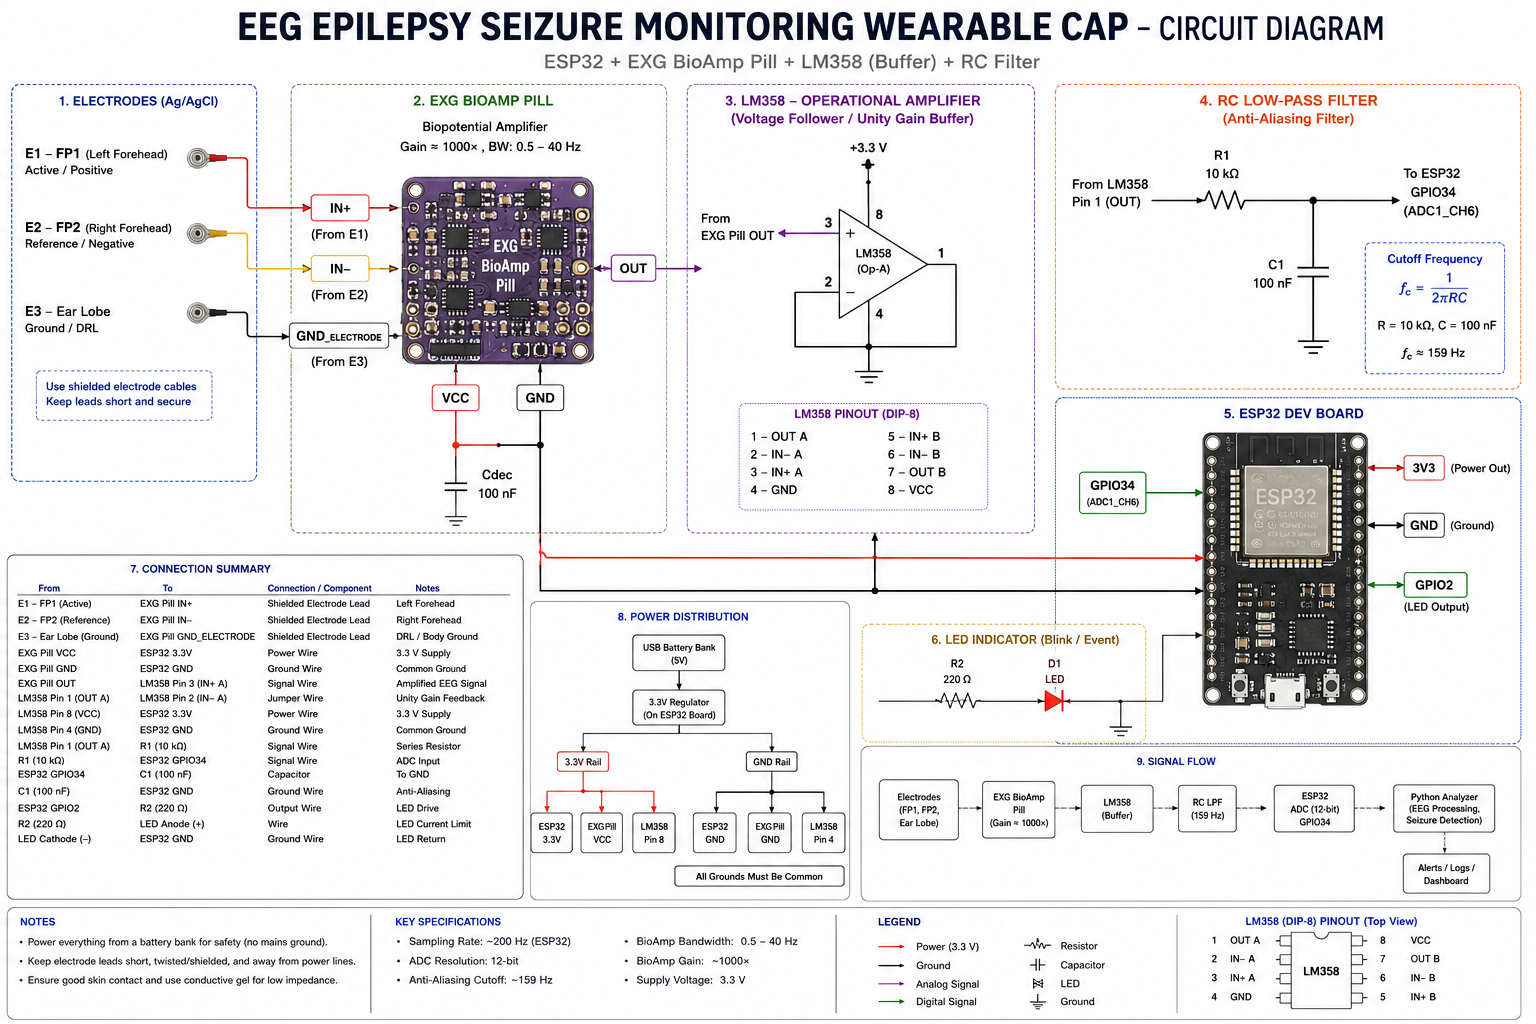
\includegraphics[width=0.92\columnwidth]{figures/circuit_diagram.png}
\caption{Prototype: Ag/AgCl electrodes (FP1+, FP2$-$, earlobe ground), BioAmp Pill, LM358 follower, RC filter, ESP32 ADC. Gain and pass-band are nominal, not measured.}
\label{fig:hw}
\end{figure}
\begin{table}[t]
\centering
\caption{Implementation status.}
\label{tab:status}
\footnotesize
\setlength{\tabcolsep}{2pt}
\begin{tabular}{>{\raggedright\arraybackslash}p{0.18\columnwidth}>{\raggedright\arraybackslash}p{0.43\columnwidth}>{\raggedright\arraybackslash}p{0.33\columnwidth}}
\toprule
Item & Specification & Status \\
\midrule
Front-end & BioAmp Pill ($\approx$1000, 0.5--40~Hz, 3.3~V), LM358 follower, RC & built; nominal; 5~V documented~\cite{bioamp} \\
ADC & 12-bit, default attenuation, \texttt{delay(5)} loop & firmware; rate not measured \\
Alerts & LED, GPIO pulse, Wi-Fi AP REST API, app & firmware; app not evaluated \\
Detectors & firmware state machine; 3-feature analyzer & replay-evaluated \\
DEV-BR & C++ header, 2.5~KB RAM & verified offline; not deployed \\
Bench data & noise, battery, cost & not measured \\
\bottomrule
\end{tabular}
\end{table}
One forehead channel (Fig.~\ref{fig:hw}) is amplified by the BioAmp Pill~\cite{bioamp}, buffered by an LM358 and digitized by the ESP32 (Table~\ref{tab:status}). The LM358 is not rail-to-rail; at 3.3~V its output tops out near 1.8~V, about 150~mV above mid-supply~\cite{lm358}.

\textbf{Shipped detectors.} The firmware tracks a baseline $b[n]{=}0.99b[n{-}1]{+}0.01x[n]$ and deviation $d[n]{=}|x[n]-\lfloor b[n]\rfloor|$, with an exponentially weighted mean $\mu$ and spread $\sigma$ (factor 0.995 per sample). Thresholds $\mu{+}2.5\sigma$ (BROWNOUT) and $\mu{+}4\sigma$ (BLACKOUT), clamped to fixed ADC ranges, are reset every 30~s, and leaky counters confirm states. A Python analyzer computes line-length (LL), delta/alpha ratio (DAR) and 30--45-Hz energy (HFE) over 2.56~s every 20 samples and requires two of three features above adaptive thresholds with fixed floors on 7 of 8 ticks.

\section{Code-Faithful Replay}\label{sec:method}
We used CHB-MIT~\cite{shoeb2009thesis,goldberger2000physionet}: all seizure recordings plus one seizure-free file per case; chb01 and chb21 are one subject. FP1--FP2 is reconstructed exactly as the signed sum of the bipolar chain FP1-F7 through FP2-F8; five files lack it, leaving \NRec{} recordings and \NSz{} seizures. Signals pass a causal 0.5--40-Hz model, are resampled to 200~Hz, scaled by gain 1000 around 1.65~V and quantized to 12~bits. The analyzer is imported \emph{unmodified} and driven by a simulated serial port and clock (5~ms per sample); the firmware \texttt{loop()} is ported line by line. Following SzCORE~\cite{dan2025szcore}, alarms within 90~s merge, a seizure is detected by an alarm in [onset$-$30~s, offset$+$60~s], and all others are false alarms. CIs use a subject bootstrap, comparisons the Wilcoxon test over 23 subjects, and chance levels \NPerm{} circular shifts of each alarm train.

\begin{table*}[t]
\centering
\caption{Event-based results on FP1--FP2 (\NSubj{} subjects, \NSz{} seizures, \NHours{}~h). Brackets: subject-bootstrap 95\% CI. ``Chance'': sensitivity of the circularly shifted alarm train. BR detectors: held-out subjects only (LOSO).}
\label{tab:main}
\begin{tabular}{lcccccc}
\toprule
Detector & Detected & Sensitivity [95\% CI] & Macro & FA/h & Latency (s) & Chance \\
\midrule
\MainTableBody
\bottomrule
\end{tabular}
\end{table*}

\section{Why the Shipped Detectors Fail}\label{sec:diag}
The analyzer's BLACKOUT alarm detected \PyBSens{} at \PyBFAh{}~FA/h; the firmware reached \FwBSens{} at \FwBFAh{}~FA/h, but its shifted alarms already reach \FwBNull{} (Table~\ref{tab:main}). Three causes emerge. (i)~\emph{Short memory}: the firmware's spread estimate forgets within about 1~s, so brief 4$\sigma$ excursions are routine. (ii)~\emph{Uninformative votes}: LL (AUC \AucLL{}) and $d$ (\AucFW{}) separate ictal from inter-ictal epochs, but DAR is at chance (\AucDAR{}) and HFE below it (\AucHFE{}), so the 2-of-3 vote waits on features without seizure information. (iii)~\emph{Absolute units}: fixed floors make detection gain-dependent (BLACKOUT \PyBSensLowGain{}, \PyBSens{}, \PyBSensHighGain{} at gains 500, 1000, 2000).

\section{DEV-BR: A Delayed-Median Ratio Detector}\label{sec:devbr}
DEV-BR addresses all three on the deviation $d$ the firmware already computes. With $t$ in seconds,
\begin{align}
\delta(t) &= \mathrm{mean}\{d[n] : n \in \text{second } t\},\\
\beta(t) &= \mathrm{median}\{\delta(\tau) : t{-}329 \le \tau \le t{-}30\},
\end{align}
and an alarm fires when $\delta \ge r\beta$ for $D$ consecutive seconds (90-s suppression, none before 330~s). The 30-s lag keeps the onset out of its own baseline, and the ratio removes the gain. $(r,D)$ is chosen by leave-one-subject-out cross-validation (LOSO): on 22 subjects we take the most sensitive setting meeting an FA/h target and apply it to the 23rd. A nested variant that also selects the signal (LL, DEV or fused) chose DEV in \NestedDev{} of \NestedAll{} folds. A header-only C++ class (330-value ring, \texttt{nth\_element} median once per second, 2.5~KB RAM) reproduced every alarm of the Python evaluation in 800 of 800 runs.

\begin{figure}[t]
\centering
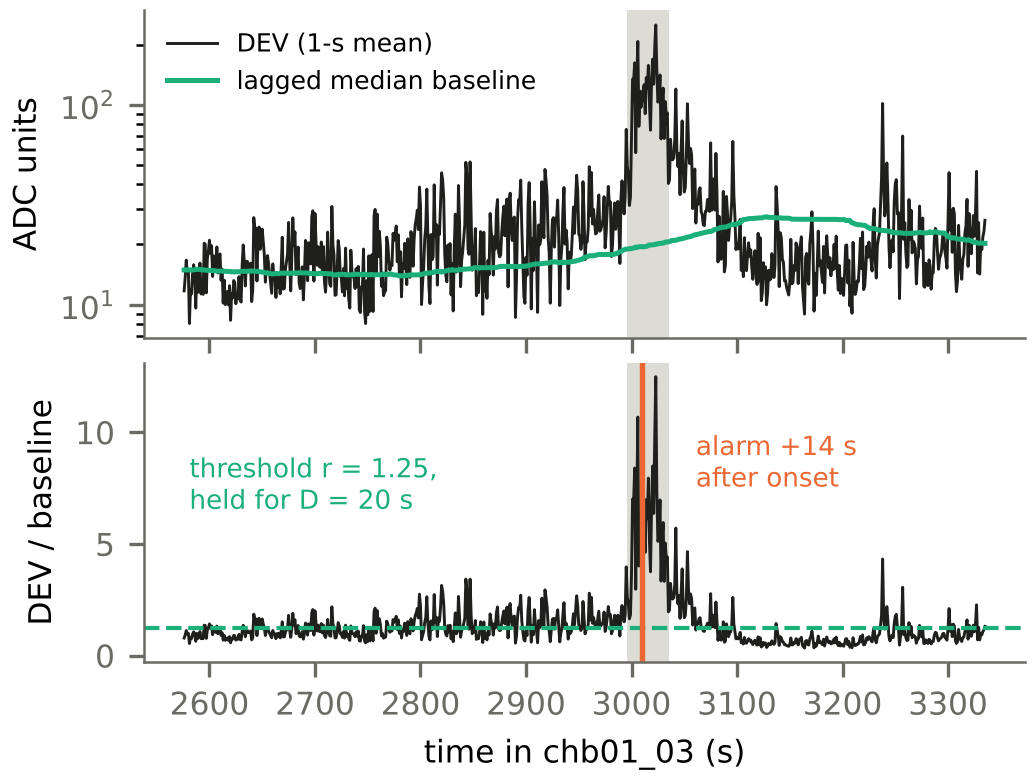
\includegraphics[width=0.9\columnwidth]{figures/devbr_example.png}
\caption{DEV-BR on a seizure in chb01 (shaded): per-second deviation and delayed median baseline (top), their ratio, threshold and alarm (bottom).}
\label{fig:example}
\end{figure}

\begin{figure}[t]
\centering
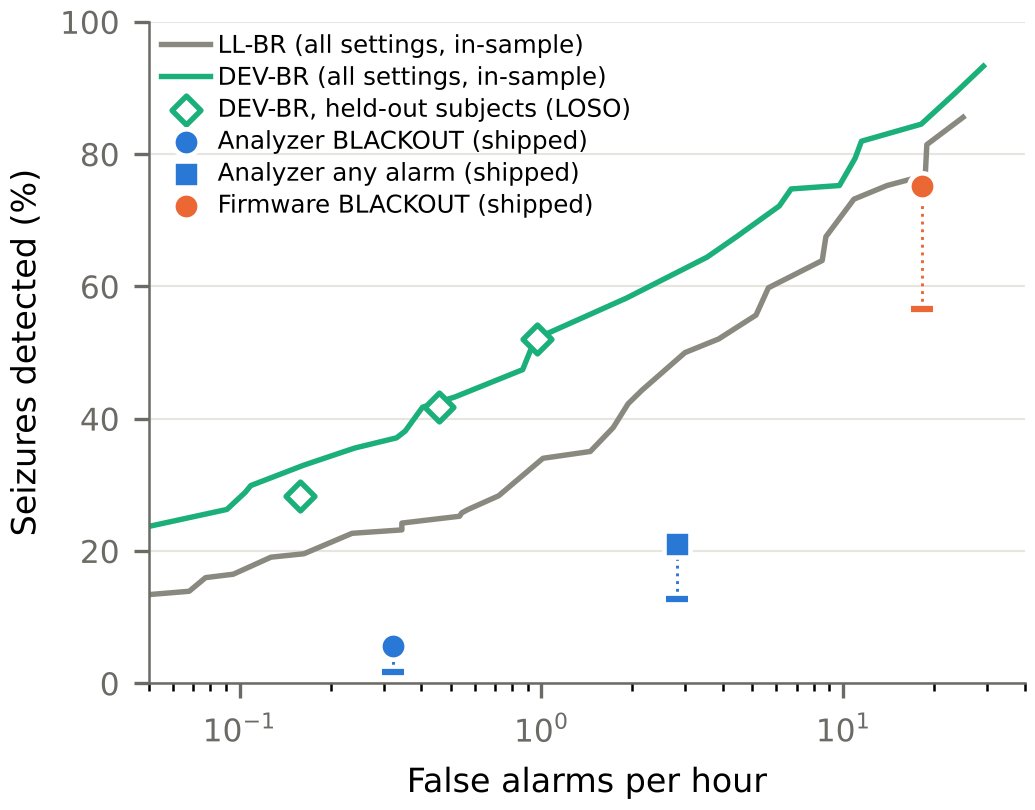
\includegraphics[width=0.86\columnwidth]{figures/operating_curve.png}
\caption{Sensitivity versus FA/h on FP1--FP2. Lines: best in-sample ratio trade-offs. Diamonds: DEV-BR on held-out subjects. Markers: shipped detectors; dashes: their chance levels.}
\label{fig:roc}
\end{figure}

\textbf{Results.} On held-out subjects DEV-BR detected \DevADet{}/\NSz{} seizures (\DevASens{}, CI \DevACI{}) at \DevAFAh{}~FA/h with median latency \DevALat{}~s, and \DevBSens{} at \DevBFAh{}~FA/h (Figs.~\ref{fig:example}, \ref{fig:roc}). That is about \FoldDevPy{} times the analyzer at a comparable alarm rate: better in \TestDevPyBetter{} of \TestDevPyN{} subjects, worse in \TestDevPyWorse{} (\TestDevPyP{}); its chance level was \DevANull{}. Without normalization the same LOSO procedure reached only \AblAbsSens{}; removing the lag or lengthening the window to 600~s also hurt (Table~\ref{tab:abl}). Excluding the \NColdStart{} seizures that begin during warm-up gives \DevASensWarm{}.

\begin{table}[t]
\centering
\caption{Ablations and alternative detectors (LOSO, FP1--FP2): sensitivity / FA/h at the $\le$1 and $\le$0.5~FA/h targets.}
\label{tab:abl}
\footnotesize
\setlength{\tabcolsep}{3pt}
\begin{tabular}{lcc}
\toprule
Variant & $\le$1 FA/h & $\le$0.5 FA/h \\
\midrule
\AblationTableBody
\bottomrule
\end{tabular}
\end{table}

\textbf{Simpler is enough.} k-of-n and dual time-scale rules, a baseline carried across files, logistic regression and gradient-boosted trees on 14 baseline-normalized features (thresholds by inner cross-validation) reached at most \AltBestOneSens{} at $\le$1~FA/h. Boosted trees gave \GbmHalfSens{} versus \DevBSens{} at $\le$0.5~FA/h, a non-significant difference (\GbmHalfP{}). Averaging or OR-ing ratios from the neighbouring frontal derivations FP1-F7 and FP2-F8 did not help either. The limit is the frontal recording site, not the rule.

\begin{table}[t]
\centering
\caption{Front-end robustness (simulated). ``Fixed'': DEV-BR with $r{=}\HwFixR$, $D{=}\HwFixD$~s chosen at gain 1000. Clip: LM358 1.8-V ceiling; Sat.: saturated samples. Cells: sensitivity / FA/h.}
\label{tab:hw}
\footnotesize
\setlength{\tabcolsep}{1.5pt}
\begin{tabular}{lcccc}
\toprule
Condition & Sat. & DEV-BR fixed & DEV-BR LOSO & Firmware \\
\midrule
\HwTableBody
\bottomrule
\end{tabular}
\end{table}
\textbf{Hardware robustness.} With parameters frozen, DEV-BR stayed at \HwDevSensMin{}--\HwDevSensMax{} and \HwDevFAMin{}--\HwDevFAMax{}~FA/h across gains, LM358 clipping (\HwClipSat{} of samples saturated at gain 2000), a 3.1-V ADC range and a 6-ms loop, while the firmware moved between \HwFwSensMin{}--\HwFwSensMax{} and \HwFwFAMin{}--\HwFwFAMax{}~FA/h (Table~\ref{tab:hw}).

\section{Discussion and Conclusion}
Replaying the code that ships showed that the prototype's on-device alarm mostly fires at random, and that a decision rule on a signal it already computes makes it a significant, hardware-robust detector at about one false alarm per hour, with no added hardware. Three principles generalize to low-cost biosignal devices: validate the shipped code, not a re-implementation; normalize against the wearer's own delayed background so decisions are invariant to front-end tolerances; and stop adding complexity once held-out tests show the signal is the bottleneck. The absolute performance is far from clinical wearables~\cite{beniczky2021guideline}, and the device is a research prototype. Limitations: results come from software replay of a pediatric clinical dataset with a nominal front-end model; non-idealities were simulated, not measured; the BioAmp runs below its documented supply; recordings start cold; and DEV-BR is not yet on the device. Next steps are bench characterization, on-device deployment, a rail-to-rail buffer, a temporal or behind-the-ear channel and an ethics-approved recording study. Hardware, firmware, analyzer, replay benchmark and C++ detector are open source~\cite{vera_repo}.

\section*{Acknowledgment}
The authors used an AI assistant (Claude, Anthropic) to help develop the evaluation code and draft the manuscript, and take full responsibility for the content.

\bibliographystyle{IEEEtran}
\bibliography{refs}

\end{document}
